
\documentclass{beamer}

\usetheme[subsectionpage=progressbar]{metropolis}

\usepackage{tikz}
\usetikzlibrary{babel}
\usetikzlibrary{arrows,shapes,positioning,shadows,trees,calc,fit}
\usetikzlibrary{overlay-beamer-styles} % 'visible on' option for nodes
\usepackage{adjustbox}


\title{Résolution de niveaux du Sokoban}
\date{\today}
\author{PoulpoGaz, darth-mole}
\institute{Candidat n° 012345}

\usepackage{graphics}
\graphicspath{{../../assets/}}
\usepackage{subcaption}

% French language support (e.g. date format)
\usepackage[french]{babel}
\usepackage[T1]{fontenc}
\usepackage{lmodern} % for missing fonts (e.g. italic in titles)

\newenvironment{customtree}{
    \begin{tikzpicture}
        [sibling distance = 10em,
        level distance = 6em,
        every node/.style = {
            shape=rectangle,
            draw,
            scale=0.85
        },
        dot/.style = {
            font = \Large
        },
        edge from parent path = {
            (\tikzparentnode) |-                          % Start from parent
            ($(\tikzparentnode)!0.5!(\tikzchildnode)$) -| % make an ortho line to mid point
            (\tikzchildnode)                              % make another ortho to the target
        }
    ]
}{
    \end{tikzpicture}%
}

\begin{document}

    \maketitle

    \begin{frame}{Plan}
        \tableofcontents%[hideallsubsections]
    \end{frame}

    \section{Le jeu du Sokoban}
        \begin{frame}{Le jeu du Sokoban}
            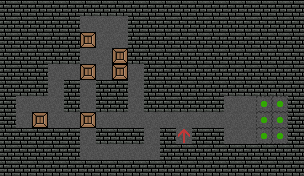
\includegraphics{Original & Extra_1.png}
        \end{frame}

    \section{Principe de résolution}
            \begin{frame}{Arbre des états}
                \begin{center}
                    \begin{tikzpicture}
                        [sibling distance=10em,level distance=6em,
                        every node/.style={shape=rectangle,draw,align=center}]

                        \node{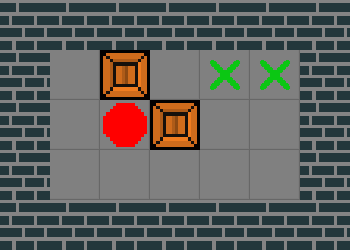
\includegraphics[width=0.2\textwidth]{exhaustive_search/1.png}}
                            child{node{\only<2-3>{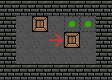
\includegraphics[width=0.2\textwidth]{exhaustive_search/2.png}}}
                                child{node{\only<3>{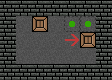
\includegraphics[width=0.2\textwidth]{exhaustive_search/5.png}}}}}
                            child{node{\only<2-3>{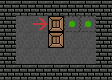
\includegraphics[width=0.2\textwidth]{exhaustive_search/3.png}}}
                                child{node{\only<3>{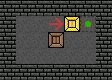
\includegraphics[width=0.2\textwidth]{exhaustive_search/4.png}}}}};
                    \end{tikzpicture}
                \end{center}
            \end{frame}

            \begin{frame}{Un graphe vu comme un arbre}
            \end{frame}

    \section{Réduction de l'espace de recherche}
        \begin{frame}{Détection de \textit{deadlocks}}
        \end{frame}

        \begin{frame}{Détection de \textit{corrals}}
        \end{frame}

    \section{Recherche dirigée par une heuristique}
        \begin{frame}{Heuristique simple \textit{(Simple Lower Bound)}}
        \end{frame}

        \begin{frame}{Heuristique gloutonne \textit{(Greedy Lower Bound)}}
        \end{frame}

    \section{Optimisations}
        \begin{frame}{}
        \end{frame}

    \section{Résultats}
\end{document}
